\section{Background and Related Works}
%\acrshort{tcp} have two basic problems. 1) \acrshort{tcp} is tightly coupled with \acrshort{ip}, 2) \acrshort{tcp}'s slow-start mechanism is ill-suited for short-lived connection. 
%To solve the first problem. i.e. decoupling \acrshort{tcp} and \acrshort{ip}, first approach is to solve it from network. So, we got Mobile IP, \acrfull{hip}, \acrfull{shim6}. These protocols try to hide the information that underlying path has been changed. It \acrshort{tcp}'s congestion control suffers from this.
%
%The another approach is to solve it from the transport layer. For this we got \acrfull{sctp} and \acrfull{mptcp}. \acrshort{sctp} is similar to \acrshort{tcp}, but it provide multi-homing and multi-path for more reliability. It is not used because it does not support \acrfull{nat} well. The application needed to add support for this protocol. It is not drop in replacement for \acrshort{tcp}. \acrshort{mptcp} is drop-in replacement for \acrshort{mptcp}. It is almost transparent to the application. If operating system support \acrshort{mptcp}, any existing application can start using \acrshort{mptcp}.
In this section, we discuss various transport protocols that are developed over the time to cope up with the changes in Internet traffic dynamics. TCP and its variants, such as~\cite{wang2014achieving,lukaseder2016comparison,wang2013cubic,de2016throughput}, are the core of the TCP/IP protocol suite. TCP provides a reliable end-to-end connection. It also takes care of the congestions in the network. However, TCP suffers from three problems -- i) it does not support mobility; 2) it does not utilize the full capacity for multi-homing; and c) it performs poorly for short-lived flows \cite{de2016throughput,islam2016start}.

To solve the problems of mobility and multihoming, researchers have come up with several solutions. These solutions can be categorized in different ways. It can be a network layer protocol (Mobile IP~\cite{MobileIp}, ECCP~\cite{arye2012formally}), a transport layer protocol (SCTP~\cite{iyengar2006concurrent}, MPTCP~\cite{mptcpsurvey}), or a combination of all (MobilityFirst~\cite{MobilityFirst,raychaudhuri2012mobilityfirst,venkataramani2014mobilityfirst}). A network consists of several different types of devices. During the development of an end-to-end protocol, it is also important to consider the heterogeneity of devices. Therefore, the development of the new protocol should also consider application level programmability and minimal changes in the existing kernel. Although MPTCP, SCTP etc. are end-to-end protocols, they need supports from middleboxes and therefore, requires significant changes at the kernel. Here we give brief design details of the important protocols that handles mobility and multi-homing. We then discuss the recent research activities in the network community to handle short flows using existing transport layer protocols. 


\subsection{Mobile IP}
Mobile IP~\cite{MobileIp} is the standard protocol to avoid IP changes for a mobile device, so that TCP connection do not need to be terminated. It is mainly an infrastructural protocol. Here mobile devices use two addresses; one is permanent home address and another care-of address. It also requires two agents to establish communication -- one home agent and one foreign agent, to forward a packet to the host. The home agent is the gateway for the home location of the device, whereas the foreign agent is the gateway through which the device get associated after it changes its location as well as the IP address.  With router-optimization, mobile IP uses triangular path, where a request is forwarded to the remote server from the mobile device; whereas the response is first forwarded to the home agent which in turns redirect it to the foreign agent via the care-of address. This type of triangular routing increases the forwarding delay for mobile IP based solution. There are several research activities going on to improve the handover from one agent to another agent for various scenarios of mobile IP based networks, such as cognitive radio network~\cite{MobileIpCognitive}, vehicular network~\cite{MobileIpVehicular2015,MobileIpVehicular2016} and commodity network~\cite{MobileIpHandover}. However, mobile IP based solution is not scalable as well as requires special infrastructure support to handle the mobility. Therefore, this types of solution has not been deployed widely over the present Internet. 

\subsection{Host Identity Protocol (HIP)}
HIP~\cite{HIP} decouples network layer and transport layer by adding a namespace layer in between them. It implements locater/identifier separation, where the identifier uniquely identifies a device, whereas the locater locates it over the Internet. HIP solves the problem of IPv4 as well as IPv6 agility, mobility, and multihoming. further, it is fully backward compatible. It also provides enhanced security. There are multiple research activities going on to improve HIP under global Internet scenario. In~\cite{HIPIoT}, the authors have shown that HIP can be used as an end-to-end secure host identity protocol for IoT. HIP can also used for providing the Internet over wireless media securely~\cite{HIPPubliceWifi}. There are researches going on to improve the mobility support as well as other features inside HIP~\cite{HIPMobility,HIPMobilityEnhanced,HIPMobilitySimulte}. However, HIP requires changes in the existing protocol stack, which limits its scalability for large scale deployment. 

\subsection{MobilityFirst Future Internet Architecture}
MobityFirst~\cite{MobilityFirst,raychaudhuri2012mobilityfirst,venkataramani2014mobilityfirst} is one of the future Internet architecture project that was funded by NSF in the year $2010$. This architecture claims to completely change the current Internet architecture considering that the end devices would be mobile devices.  few of the advanced features that are supported over MobilityFirst architecture as as follows -- a)separation of naming from addressing, b) security and global identifier, c) global name resolution service, d) storage-aware delay tolerant routing, e) mobility, and f) context aware networking~\cite{MobilityFirstContextAwareDemo}. The various design goals for the MobilityFirst project are as follows.
\begin{enumerate}
	\item[G1.] \textbf{Host and network mobility}: The target is to ensure an end-to-end communication despite of frequent mobility of the end hosts or networks; as well as to support communication during the absence of a contemporaneous end-to-end path.
	\item[G2.] \textbf{No global root of trust}: MobilityFirst assumes that the correct network behavior does not depend on a single root of trust. 
	\item[G3.] \textbf{Intentional data receipt}: Under MobilityFirst architecture, an end-host receives data only if the transmission is consistent with its receipt policy.
	\item[G4.] \textbf{Byzantine robustness}: MobilityFirst supports Byzantine robustness, which ensures the an end-to-end communication can continue under the compromise of a small fraction of end-hosts or infrastructural nodes.
	\item[G5.] \textbf{Content addressability}: Under MobilityFirst architecture, the network assists in content retrieval apart from host-to-host communication.
	\item[G6.] \textbf{Evolvable network services}: MobilityFirst architecture allows for the co-existence of various network services.
\end{enumerate}
However, MobilityFirst requires multiple changes over the current Internet architecture to support seamless mobility of host devices during data communication. 

\subsection{End-to-end Connection Control Protocol (ECCP)}
ECCP~\cite{ECCP} is a transport layer protocols that puts a layer abstraction below the transport layer, similar to Mobile IP. However, unlike mobile, it does not try to hide the underlying network changes to TCP connection. It just maintains the abstraction as long as needed. An ongoing connection continues as long as it exists. ECCP does not put any limitation on the protocol to be used. It also creates flows like MPTCP, but this flow can be reused. It supports multipath and multihoming. 

There are some other protocols to support mobility over the Internet, like TCP-Migrate, Locater/Identifier Separator Protocol (LISP)~\cite{LISPRFC6830}, I3~\cite{I3-internet-indirection-infrastructure} etc., which provide a solution for seamless data communication during host mobility. However, the overhead for these protocols are high, and also they require significant changes in the TCP/IP protocol stack. Another group of solutions for mobility uses name servers to resolve the host IP during mobility, which includes eXpressive Internet Architecture (XIA)~\cite{XIA}, Named Data Networking (NDN)~\cite{ndn}, msocket~\cite{Yadav2016} etc. However, these protocols does not handle traffic divergence over the network, and known to be performed poorly for short flows~\cite{dukkipati2006flow}.

\subsection{Stream Control Transfer Protocol (SCTP)}
SCTP~\cite{RFC4960} is a transport layer message-based multi-streaming protocol. It is UDP like message-oriented, and it ensures end-to-end reliability. Unlike the previous protocols that support mobility over the Internet, SCTP is an easy to deploy protocol. In the event of unavailability of native support of SCTP, UDP encapsulated SCTP~\cite{RFC6951} can also be used. The advantages of SCTP over TCP is that it supports multihoming delivery at both the ends. The packet transfer mechanism also eliminates head-of-the-blocking. However, many NAT boxes and routers discard SCTP packets as they cannot handle them. This is one of the reasons that SCTP is not widely used in today's Internet.

\subsection{MultiPath TCP (MPTCP)}
Now a days, many of the end devices support multiple interfaces, like cellular and Wi-Fi interfaces. With the advent of smartphones and smart devices that uses multi-interface supports for data communication, we observe an increased interest among the Internet researchers to utilize several interfaces in the same connection, so that it becomes possible to use both the interfaces simultaneously, and the connection can be transparently changed from one to another in the case of any failures. Further, use of multiple simultaneous path can improve the end-to-end capacity between the two end hosts. MPTCP~\cite{mptcpsurvey} is a variant of TCP that uses such multiple simultaneous connections between two hosts to support better capacity and failure recover. As MPTCP is one of the important baseline protocol for our research, here in this section, we give a detailed description of its working procedure. 


\subsubsection{Transpor Layer Structure}

MPTCP splits the transport layer into two sublayers as shown in Fig.~\ref{fig:TransportLayerStructure} ~\cite{barreia2014multipath}. The top sublayer is responsible for acquiring the necessary information to manage the connection that operates end-to-end. The bottom sublayer is responsible for the sub-flows to operate as a single TCP flow, and allows the TCP components to operate simultaneously. This structure is designed to be transparent to both the top and the bottom layers. To manage the MPTCP sub-flows, the bottom sublayer of the transport layer needs to implement additional functionalities, like packet scheduling, path management, sub-flow interface and congestion control mechanisms.

\begin{figure}[!ht]
    \centering
    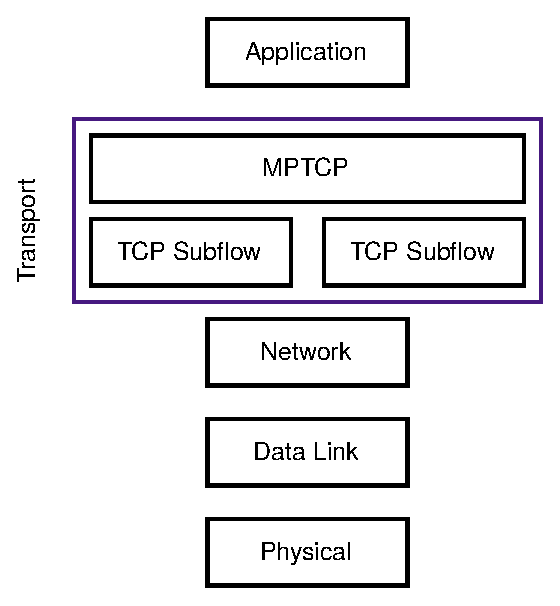
\includegraphics[width=.5\textwidth]{img/mptcp/mptcp_str}
    \caption{Transport Layer Structure for MPTCP~\cite{barreia2014multipath}}
    \label{fig:TransportLayerStructure}
\end{figure}

Here we give a brief description and functionalities of various modules of MPTCP. The \textbf{path management} module in MPTCP is responsible for finding and using the available paths between two end hosts. This module is also responsible for the advertisement of other alternative addresses to the end hosts and to set up new sub-flows.
The \textbf{packet scheduler} module divides the byte stream received from the applications into segments to transmit them on any one of the sub-flows available. Also in this module, the connection level re-ordering is performed whenever the packets are received from the TCP sub-flows. The \textbf{congestion control} module is responsible for coordinating between the sub-flows to maintain the congestion control mechanism. This coordination is responsible for scheduling segments between various sub-flows and controls the transfer rate. The \textbf{sub-flow interface} is in charge of transmitting the segments received from the packet scheduler on a specified path. On receipt of a segment, it passes the data to the packet scheduler for connection-level reassembly. Since MPTCP underneath uses TCP for network compatibility, it ensures reliable and in-order delivery.

\subsubsection{Connection Handling in MPTCP}
To establish a new connection, an application has to open a TCP socket, which will enable the initial TCP sub-flow. After the initial TCP connection, if both the hosts support MPTCP capability, the MPTCP session can start on both the end hosts. The connection set up procedure is  shown in Fig.~\ref{fig:ConnectionHandling}~\cite{barreia2014multipath}.
To establish a new sub-flow from the one host, say host A, to another host, say host B, host A receives the IP address of one of the interfaces of host B from the name server. A three-way handshake mechanism is used for connection establishment, which is similar to normal TCP, but it carries MPTCP specific informations in the additional header fields, which are only interpretable by the MPTCP supported end systems. The MP\_CAPABLE option is added on the handshake to allow both the hosts to inform each other that they support MPTCP capability, as explained in Fig.~\ref{fig:ConnectionHandling}. The MPTCP connection initiation ends at this point, and the end hosts then set up the sub-flows as explained next. 

\begin{figure}[!ht]
    \centering
    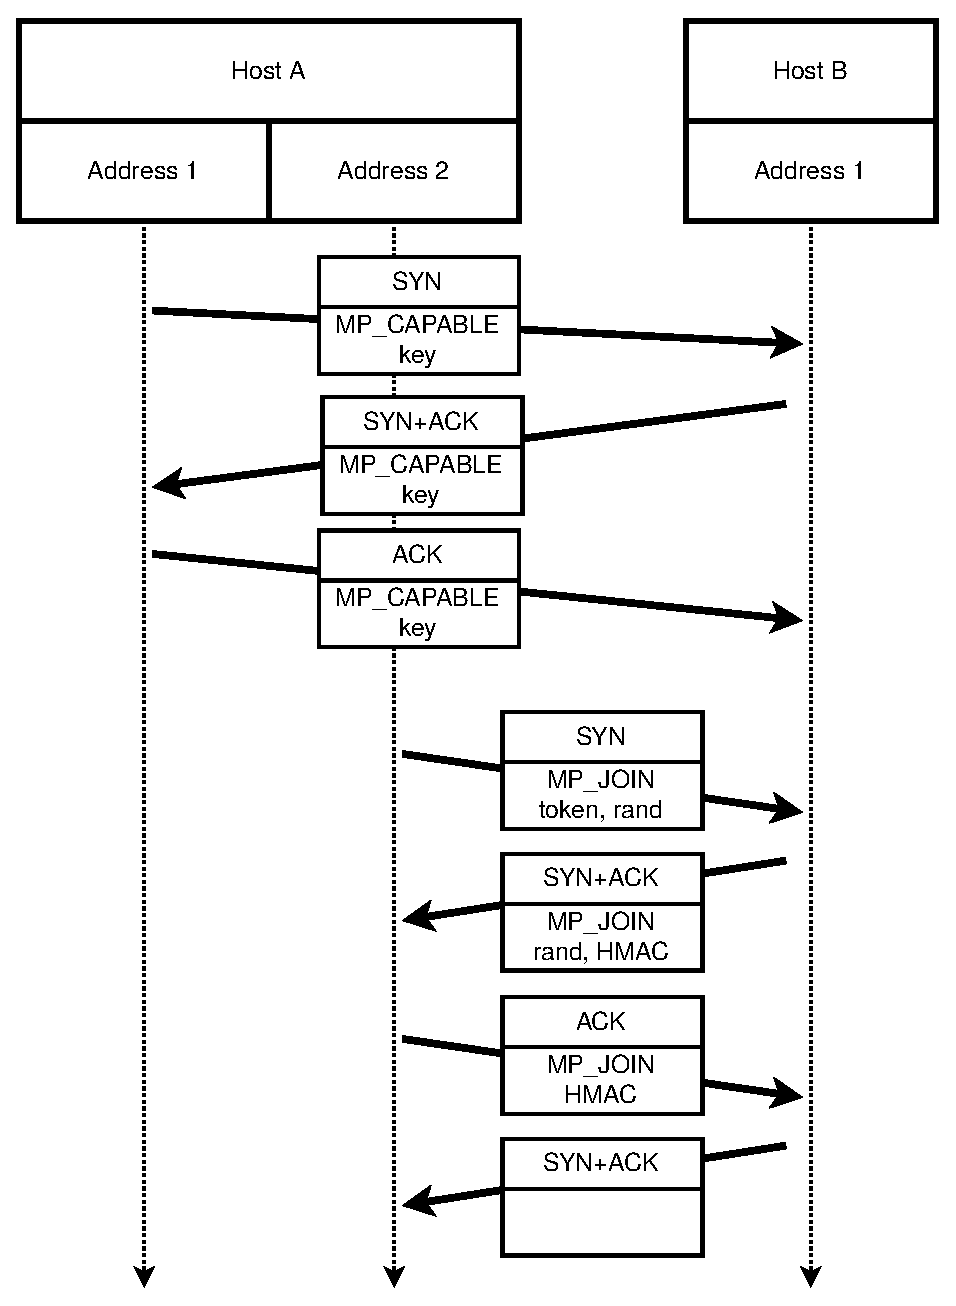
\includegraphics[width=.5\textwidth]{img/mptcp/mptcp_con}
    \caption{Three Way handshaking for Connection Establishment between MPTCP Supported Hosts}
    \label{fig:ConnectionHandling}
\end{figure}

Assume that host A wants to create a sub-flow between its second interface (say, with IP address A.2) and host B's default interface (say, with IP address B.1). Again a new TCP three-way handshake starts, but the option in use is different because the new sub-flow needs to be attached to the existing MPTCP session. The option that will be used to build new sub-flows is MP\_JOIN. Host A can establish a new sub-flow using the addresses <A.2,B.1>.
However, this sub-flows need to be attached with the existing MPTCP session between the two hosts. To achieve this, host A attaches a token for host B to the MP\_JOIN option, that identifies the existing MPTCP session. Host B responds with \texttt{SYN} and \texttt{ACK}, with MP\_JOIN option without a token, because host A already has a state for that sub-flow. Then host A sends \texttt{ACK} with the MP\_JOIN, in the context of host B. Then host B sends the final ACK, and the sub-flow is ready to be used.

It can be noted that MPTCP first initiates the connection between the two end hosts at their default interfaces, which is known as the \textit{primary path}. Once the primary path is established, the MPTCP supported hosts for additional or alternate paths via different interfaces. These paths are known as \textit{alternate paths}. Therefore, a MPTCP connection is first established over the primary path, and then it gets extended over the alternate paths. 

%MPTCP\cite{scharf2013multipath} is a recent drop in replacement for TCP. It is backward compatible, transparent to the application protocol. MPTCP supports mobility and multihoming. MPTCP utilize multiple network interface available to a device to speed up data transfer rate. MPTCP is just an extension of TCP\cite{mptcpsurvey}. It adds MPTCP layer on top of TCP and provides a congestion control algorithm. Normal TCP is a variation of MPTCP with a single sub flow. There are several challenges in designing the congestion control algorithm for MPTCP.
%%MPTCP is designed with these 
%
%\subsubsection{The Architectural Priciples}
%Application connects using regular socket API. MPTCP manages underlying TCP connections called sub-flow. Subflow is responsible for transferring data between hosts. MPTCP acts as a sub-layer in the stack shown in Fig.~\ref{fig:mptcpstack}. MPTCP uses additional signal using TCP optional header.
%
%\begin{figure}[h!]
%\centering
%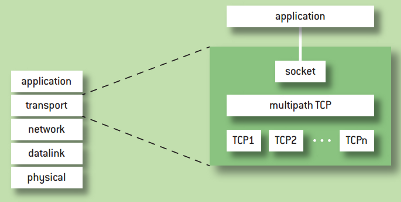
\includegraphics{img/mptcp/paasch1}
%\caption{MultiPath TCP in the TCP/IP Stack}
%\label{fig:mptcpstack}
%\end{figure}
%There are three phases in MPTCP:
%\begin{enumerate}
%    \item Connection Establishment
%    \item Add new sub-flow
%    \item Transmit data on the MPTCP connection.
%\end{enumerate}
%
%\textbf{Connection Establishment:}
%MPTCP establishes a connection using normal TCP's three-way handshaking. During connection establishment phase, MPTCP adds $MP_CAPABLE$ option with it the $SYN$ packet. If the server has MPTCP supported then it adds a $MP_CAPABLE$ option with the $SYN+ACK$ packet. And final $ACK$ packet also contain $MP_CAPABLE$ option. MPTCP (server or client) add a random key for security with its $SYN$ packet. 
%
%\begin{figure}[h!]
%\centering
%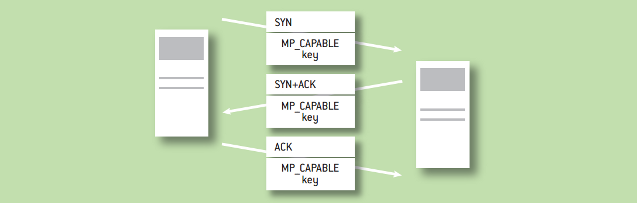
\includegraphics[width=\linewidth]{img/mptcp/paasch2}
%\caption{Three-way handshaking to establish MPTCP connection}
%\label{fig:ConnectionEstablishment}
%\end{figure}
%Three-way handshaking is shown in Fig.~\ref{fig:ConnectionEstablishment} create one MPTCP sub-flow to an interface. To use another path, MPTCP needs to add another sub-flow using a three-way handshake. However, this sub-flows need to be identified properly. Normal TCP identified by 4 tuple of $<src_ip,dst_ip,src_port,dst_port>$. MPTCP cannot use this as this tuple is host dependent. And network middlebox like NAT can change them. So MPTCP needs something more. 
%
%\begin{figure}[h!]
%    \centering
%    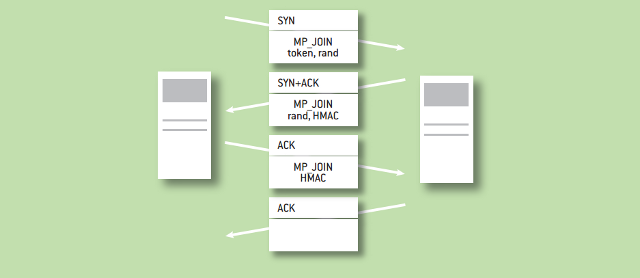
\includegraphics[width=\linewidth]{img/mptcp/paasch3}
%    \caption{}
%    \label{fig:4way}
%\end{figure}
%
%\textbf{Create additional sub-flow:} MPTCP uses 4 way handshaking shown in Fig.~\figurename{fig:4way} to add sub-flow. To add extra sub-flow, MPTCP uses the $MP_JOIN$ option with a $SYN$ packet. The $MP_JOIN$ option used to authenticate the sub-flow. Here $token$ is the truncated hash of key it receives during $MP_CAPABLE$ exchange. In this phase, two parties first exchange random nonce and then it compute HMAC based on the nonce and forward it to another party. Once both parties receive the $ACK$ for the random nonce it shared, the sub-flow is established.

\subsubsection{Data Transfer and Congestion Control}
Once all the sub-flows are added, data can be transmitted between two hosts via multiple paths. MPTCP uses a congestion control algorithm, however, a straightforward extension of the TCP congestion control algorithm may perform poorly when the same session is shared over multiple paths. Paas \textbf{et. al.}~\cite{PaaschMptcp} have suggested a simple solution by using independent TCP congestion control for each path. However, their results show that MPTCP captures most of the bandwidth in a link that affects other ongoing communications over the shared paths. Accordingly, new congestion control algorithms have been proposed for MPTCP, as discussed next. 

\textbf{Link Increases Algorithm (LIA)}: As mentioned that using the normal TCP congestion control algorithm at both the paths of MPTCP affects other independent TCP connections that share the path. Therefore, Raiciu \textit{et. al.}~\cite{LIARFC6356} have proposed a new congestion control algorithm, called {\em Link Increases Algorithm} (LIA) to couple multiple paths, and use an aggressiveness factor to control the subflow window increment. The congestion window tuning mechanism without the aggressive factor is as follows. For each \texttt{ACK}, MPTCP increase the congestion window ($w_r$) by the following factor. 
$$w_{r+1} = \min\left( \frac{\max\limits_{i \in \mathcal{R}_u} w_i/rtt_i^2}{\left(\sum_{i \in \mathcal{R}_u}w_i/rtt_i\right)^2}, \frac{1}{w_r}\right) $$
Here $\mathcal{R}_u$ is the set of paths available to the MPTCP sender $u$. $w_r$ and $rtt_r$ are the congestion window size and the RTT, respectively, at path $r \in \mathcal{R}_u$. On reception of a packet, the congestion window is decreased as follows.
$$w_{r+1} = \frac{w_r}{2}$$


\textbf{Opportunistic Linked-Increases Algorithm (OLIA):} In MPTCP, all the sub-flows may not go through a distinct path. It may happen that two or more sub-flows have overlapped path that may create bottleneck at the end-to-end flow. LIA tries to balance the congestion between the two available paths. However, as paths are same, these two sub-flows start behaving like individual TCP flows. This results in unfairness to other normal TCP flows, as MPTCP may grab more share of the bottleneck bandwidth. So LIA is not Pareto optimal~\cite{OLIARamin2012}. Khalili \textbf{et. al.}~\cite{OLIARamin2012} have propose a modification to the LIA algorithm named as \textit{Opportunistic Link Increases Algorithm} (OLIA). The congestion window tuning mechanism for OLIA works as follows.  On the reception of an \texttt{ACK} packet, the congestion window is increased as follows. 
\begin{equation}
w_r = \frac{w_r/rtt_r^2}{\left( \sum_{p \in \mathcal{R}_u}w_p/rtt_p\right)^2} + \frac{\alpha_r}{w_r}
\end{equation}
where,
\begin{equation}
\alpha_r = \left\lbrace 
\begin{array}{ll}
\frac{1/|\mathcal{R}_u|}{|\mathcal{B}\smallsetminus \mathcal{M}|}  &\mbox{if} \hspace{0.3cm} r \in \mathcal{B}\smallsetminus\mathcal{M}\neq\emptyset   \\
- \frac{1/|\mathcal{R}_u|}{|\mathcal{M}|} \hspace{1cm}&\mbox{if} \hspace{0.3cm} r \in \mathcal{M} \hspace{0.3cm}\mbox{and}\hspace{0.3cm}\mathcal{B}\smallsetminus\mathcal{M}\neq \emptyset \\
0 & \mbox{otherwise}
\end{array} \right. 
\end{equation}


\textbf{Balanced Linked Adaptation for Congestion Between MPTCP and Normal TCP}:
LIA and OLIA  suffer from the problem of unfair bandwidth allocation when it bottlenecks with the normal TCP flows. Walid \textit{et. al.}~\cite{walid2015balanced} have presented another variant of MPTCP congestion control algorithm, called {\em Balanced Linked Increases Algorithm} (BALIA). BALIA balances the trade off between TCP-friendliness and algorithmic responsiveness in MPTCP.

\subsubsection{Current Researches on MPTCP Performance Improvement}

MPTCP uses coupled congestion control algorithm which is also known as LIA~\cite{LIARFC6356}. However, LIA is not Pareto optimal~\cite{OLIARamin2012}. It decreases the bandwidth utilization of other TCP flows on the Internet. So Khalili \textit{et. al.}~\cite{OLIARamin2012} suggested using OLIA, as a new and more conservative congestion control algorithm for MPTCP to avoid the aggressive behavior. Ferlin \textit{et. al.}~\cite{MPTCP-SBD} have argued that OLIA is more conservative, and may under-utilize the link capacity when the two paths do not share a common bottleneck. Accordingly, they have developed a mechanism to detect shared bottleneck among multiple MPTCP paths, called MPTCP-SBD. The conservative congestion control algorithm can be applied only when there is a shared bottleneck between the two paths. 

Currently, the available congestion algorithms for MPTCP are LIA, OLIA, BALIA and wVegas\cite{wVegas}. Apart from wVegas, all are \texttt{ACK} driven algorithm. Gonzalez \textit{et. al.}\cite{Balia-wvegas} have suggested a hybrid algorithm using the delay as well as the \texttt{ACK}. A number of recent researches, such as~\cite{aschedulermptcp,blestschedular,scheadulerformptcp}, have shown several ways of scheduling a packet over MPTCP paths. 

However, MPTCP is known to perform poorly for short lived flows, when a small amount of data needs to be transmitted. Hwang \textit{et. al.}~\cite{scheadulerformptcp} have suggested that for small data transmission, it is better to use single path, rather than using multipath, as MPTCP takes additional time to set up the sub-flows through the alternate paths. As flows can go through a heterogeneous path, it may cause head-of-line blocking. Therefore, in~\cite{blestschedular}, the authors have developed a predictive scheduling algorithm, called BLEST, that reduces the head-of-line blocking. Other than congestion control algorithm and scheduling algorithm, researches has been done in combined congestion control algorithm~\cite{outofordermptcp}, performance tuning~\cite{optimization},] and multimedia streaming~\cite{streaming} over MPTCP.


\subsection{Transport Protocols for Handling Short Lived Flows}

None of the above solutions have addressed the issue of short-lived connections. A large part of the traffic on the Internet uses short-lived connections~\cite{kheirkhah2015short}. A short-lived connection does not last enough to get out of the slow start phase in TCP congestion control, and therefore does not able to utilize the complete capacity of the network. It is a problem for the web servers and middleboxes like routers near to heavily loaded web servers, that need to retain the connection and associated resources for long time. 

To address this issue, Dukkipati \textit{et. al.}~\cite{google-long-initcwnd} from Google have suggested to increase the initial congestion window size to least $10$ MSS from $1$ MSS, where MSS is the maximum segment size of the TCP connection. In general, it takes up to $3$ RTTs to reach the congestion window to $10$ MSS. For short flows like web browsing, Most of the time it does not have enough data to transmit after $4$ RTTs. TCP also take $1.5$ RTT during connection establishment phase for three-way handshaking. In~\cite{google-fast-open}, Radhakrishnan \textit{et. al.} have suggested that we should also send data during the connection establishment phase, which can save resources for short flows over the Internet. However, such solutions are also not enough for short-lived connections over a long-fat link that have high bandwidth support. Web browsers produces a very larger number of short-lived flows. Each of those flows goes through separate single TCP connections. Consequently, there are multiple works that address the issues of short flows in the Internet, as we discuss next.

\subsection{SPDY}
As a part of Google's ``Let make the web faster" initiative, SPDY has been developed as an experimental protocol~\cite{spdy}. SPDY offers a way to make the web faster from controlling the link parameters from the application layer. The goals of SPDY are as follows.
\begin{itemize}
    \item SPDY promises an overall reduction in 50\% of page load time.
    \item SPDY targets to support easy deployability. SPDY uses TCP as the underlying transport protocol, so it does not require to change the existing TCP/IP protocol stack.
    \item It should not require any changes in the web content. i.e. it should be transparent to both the user and the website developer.
\end{itemize}

\subsubsection{Design and Features}
SPDY adds an extra session layer on top of normal secure socket layer (SSL) layer of HTTPS, as shown in Fig.~\ref{fig:spdy.design}. SPDY does not change usual HTTP methods like GET or POST. However it add its own frame format for encoding and data transmission. 
\begin{figure}[!ht]
    \centering
    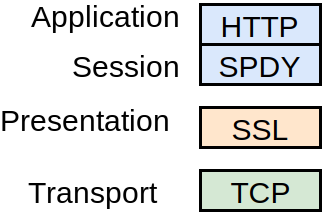
\includegraphics[width=0.2\linewidth]{img/spdy/spdy_design}
    \caption{SPDY Design}
    \label{fig:spdy.design}
\end{figure}
SPDY is a multiplexed stream base protocol where the streams are bi-directional. SPDY aims to achieve low latency through basic and advanced features as discussed next.

\noindent \textbf{Basic features:} The basic features of SPDY are as follows. 
\begin{itemize}
    \item \textbf{Multiplxed Streams}: It multiplexes multiple streams over a single TCP connection between the server and the client. It uses concurrent transmission of streams.
    \item \textbf{Request Prioritization:} Client can request as many objects as it wants from the server. However, it may happen that one stream is clogging the connection. So, SPDY provides an option to give prioritization between streams so that it can block some streams at the time of congestion.
    \item \textbf{HTTP Header Compression:} SPDY compresses request and response headers resulting in less number of bytes in transmission.
\end{itemize}

\noindent \textbf{Advanced features:} The advanced features of SPDY are as follows. 
\begin{itemize}
    \item \textbf{Server Push:} SPDY have an option to push objects to the client before it even asks for. It is useful in case of loading a page for the first time. Standard HTML page contains huge number objects to enrich the browsing experience. In this case, the server knows what the client is going to ask for, but the client may require time to process the page, and then ask the content from the server. Push will help in enriching the experience by putting in the tip of client's finger.
    \item \textbf{Hint:} Server Push is useful, however, a client may not require all of the objects as it may be in their cache. So, SPDY provides a header filed to tell the client what are the object it is supposed to ask and the server will be ready to serve those.
\end{itemize}
SPDY is a session layer protocol. It maintains a persistent TCP connection called session between the server and the client. Then it send multiple streams in interleaved fashion, as shown in Fig.~\ref{fig:http-timing-diagram}.

\begin{figure}[h]
    \centering
    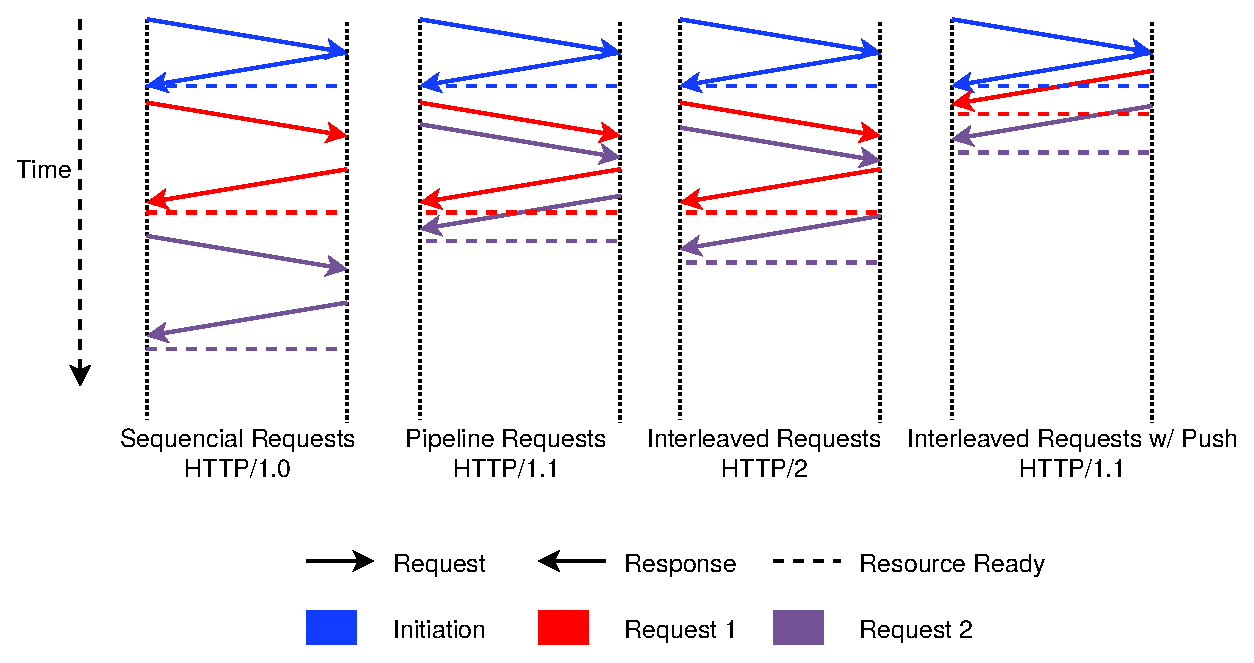
\includegraphics[width=0.8\linewidth]{img/spdy/http-timing-diagram}
    \caption{Comparison of Time to Fetch a HTTP Request}
    \label{fig:http-timing-diagram}
\end{figure}


%To solve this Google introduced experimental protocol SPDY\cite{spdy}. To avoid slow-start phase, Google multiplexed a large number of connection through a single TCP connection. SPDY become the standard from HTTP/2.0.
In~\cite{howspeedis}, Wang \textit{et. al.} have shown that uses of SPDY performs better with short-lived connections. SPDY decreases the retransmission count. However, SPDY hurts under high packet loss as it uses single TCP connection and that TCP connection decreases its window size drastically.  Eikhatib \textit{et. al.}~\cite{canspdymake} have shown that SPDY works better only when a browser has to fetch large numbers of small files from the server. Chinnaga \textit{et. al.}\cite{scalabilitySPDY} have developed tool to test SPDY's perform. In~\cite{han2015anatomy}, the authors have explained how SPDY's performance can be improved using MPTCP.

Interestingly, SPDY goes back to the OSI protocol stack from the TCP/IP protocol stack by presenting the session layer after application layer. Although SPDY gives a direction to revisit the end-to-end protocol design fundamentals, it suffers from the head-of-line blocking problem. If one TCP packet gets lost in the network, TCP does release rest of the packets, until it recovers the lost packet. As SPDY is a stream multiplexing protocol, all the streams have to wait for the lost packet. Further, SPDY does not support mobility as the underline TCP protocol does not support mobility. To overcome these issues, Google have developed the next version of the end-to-end protocol for future Internet, called Quick UDP Internet Connections (QUIC).

\subsection{Quick UDP Internet Connections (QUIC)}
Quick UDP Internet Connections (QUIC) is an experimental protocol developed by Google. It is designed to provide
security and reliability along with reduced transport latency. Google has already deployed QUIC protocol on their servers and has a client implementation in their web browser, Chrome. We have shown a comparison with HTTP/2 in the layering approach in Fig.~\ref{fig:quic-protocolstack}. It is built on the top of UDP. QUIC itself contains the congestion control and loss recovery like TCP. The advantage of QUIC is that it provides encapsulation of the complete TLS and HTTP combined, and does provide end-to-end security.

\begin{figure}[!ht]
    \centering
    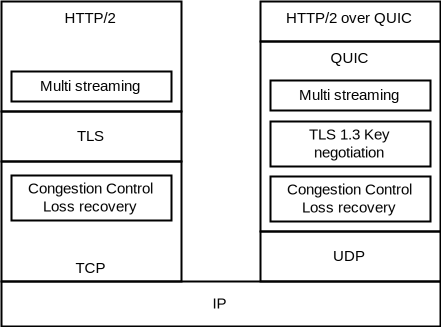
\includegraphics[width=0.6\linewidth]{img/quic/quic-protocolstack}
    \caption{QUIC Protocol Stack}
    \label{fig:quic-protocolstack}
\end{figure}

\begin{figure}[!ht]
    \centering
    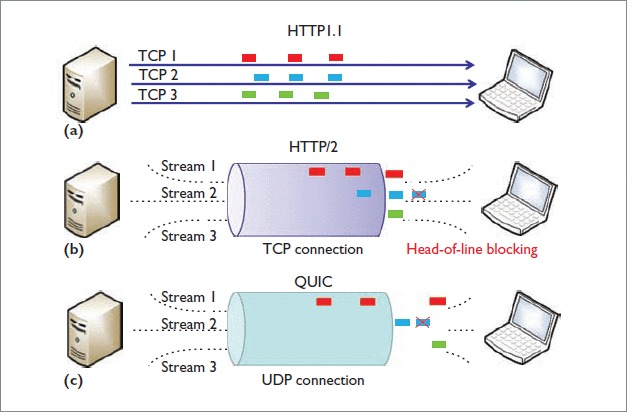
\includegraphics[width=.8\textwidth]{img/quic/transmission_compare}
    %    \includegraphics[width=.6\textwidth]{quick1}
    \caption{Flow Multiplexing in QUIC~\cite{carlucci2015http}}
    \label{fig:Quic1}
\end{figure}

QUIC multiplexes several streams over the same UDP connection. Fig.~\ref{fig:Quic1}~\cite{carlucci2015http} shows that with HTTP/1.1, a client can only use one resource at a time; whereas with QUIC, a client can send multiple HTTP requests and receive multiple responses over the same UDP socket. HTTP/1.1 web browsers attempt to minimize the impact of the head of the line blocking by opening multiple concurrent HTTP connections, typically up to
six. The QUIC multiplexing feature has been inherited from SPDY.

\begin{figure}[!ht]
    \centering
    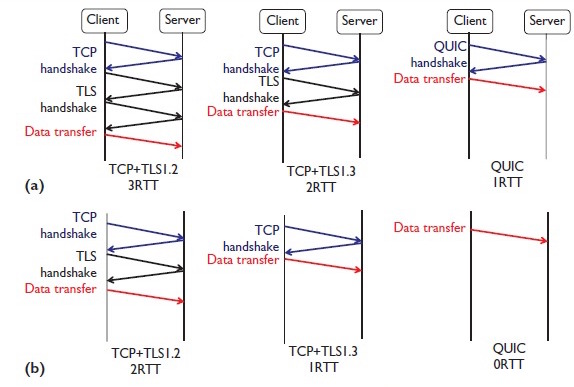
\includegraphics[width=.9\textwidth]{img/quic/quicrrtcompare}
    \caption{Connection Establishment for Different Protocols~\cite{quicisquic}}
    \label{fig:Quic2}
\end{figure}

One of the important features of QUIC is that it can connect to a client with 0-RTT, if there is already an ongoing connection between them. This can reduce the huge overhead of reconnection compared to TCP dependent protocols. Fig.~\ref{fig:Quic2}~\cite{quicisquic} clearly shows the way QUIC and other protocols differs based on their connection establishment procedures. 
%
%\begin{figure}
%    \centering
%    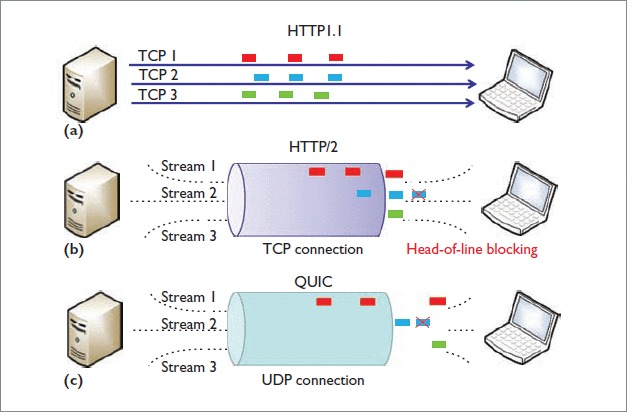
\includegraphics[width=.6\textwidth]{img/quic/transmission_compare}
%    \caption{Comparison of connection RTT.}
%    \label{fig:connectiontime}
%\end{figure}
%QUIC\cite{quic} is another experimental transport protocol developed by Google on top of UDP to make the web faster. Like SPDY it is also a stream multiplexing protocol, But it uses UDP as the underlying protocol. As UDP does not provide reliability or congestion control and flow control, it handles them by itself only. By providing congestion control by itself, it overcomes the problem of head-of-the-blocking. QUIC does not use any IP: Port as a connection identifier. It uses some unique identifier as a connection identifier. It helps QUIC in achieving Mobility.
%
%QUIC need 1 RTT time for connection establishment for the first time. After that, it can reuse the existing connection and archives 0RTT connection establishment. 

In \cite{quicmakewebfast}, Biswal \textit{et. al.} have experimentally found that QUIC loads pages quicker than HTTP/2 under poor network conditions. QUIC's performance also increases with the increase in object size and number of objects on a page. Megyesi \textit{et. al.}~\cite{quicisquic} have presented a comparison study of QUIC, SPDY, and HTTP. They found that QUIC can load pages faster than HTTP. However, they also concluded that HTTP works better for large object size. It can be noted here that QUIC does not support multiple paths inherently, and therefore, cannot utilize the full capacity of the network. 

\subsection{Summary}

In a nutshell, we observe that although the current researches have focused in developing new protocols to support end-to-end functionalities based on the future Internet architecture, they still lacks several design requirements. While MPTCP is known to perform poorly for short flows, QUIC does not support multihoming inherently. Therefore, in this research work, we target to revisit the end-to-end protocol design goals and plan to develop a complete solution to support device as well as application heterogeneity, while ensuring application level programmability. Based on our study of the existing protocols, the various design requirements for developing an end-to-end protocol for the next generation Internet are as follows;
\begin{enumerate}
	\item Support of device and application heterogeneity,
	\item End-host mobility, 
	\item Traffic heterogeneity -- performance should be comparable for both short flows and longs flows over the Internet,
	\item Better utilization of network capacity through multihoming,
	\item Reliability and security,
	\item Scalability,  
	\item Modular architecture and application programmability.
\end{enumerate}  
In the next section, we analyze the existing MPTCP protocol in details, considering it as the baseline for the development of the new end-to-end protocol. 